\documentclass{article}
\usepackage{tikz}
\usepackage{hyperref}
\usepackage{xcolor}

\hypersetup{
  colorlinks=true
}

\usetikzlibrary{intersections}

\begin{document}
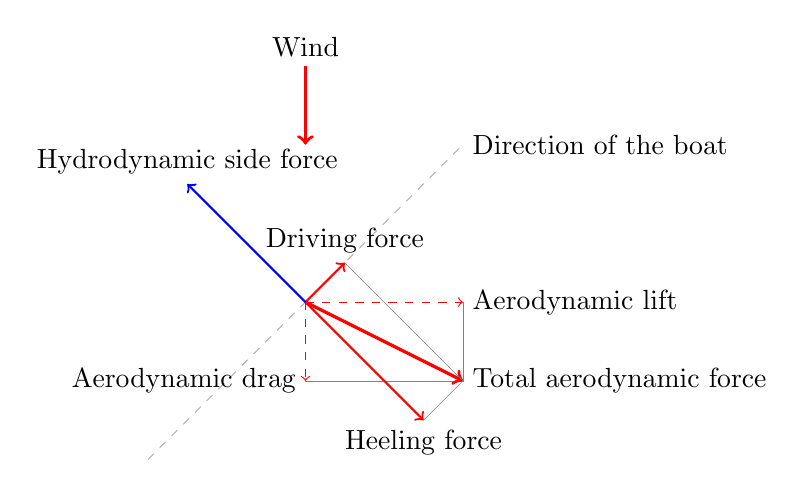
\begin{tikzpicture}
  % Boat
  \draw[help lines, dashed] (-2,-2) -- (2,2);
  \node[above, right] at (2,2) {Direction of the boat};

  % Wind
  \draw[very thick, red, ->] (0,3) -- (0,2);
  \node[above] at (0,3) {Wind};

  % Aerodynamic forces
  \draw[red, dashed, ->] (0,0) -- (2,0);
  \node[right] at (2, 0) {Aerodynamic lift};

  \draw[red, dashed, ->] (0,0) -- (0, -1);
  \node[below, left] at (0, -1) {Aerodynamic drag};

  \draw[help lines] (0, -1) -- (2, -1) -- (2, 0);
  \draw[very thick, red, ->] (0,0) -- (2, -1);
  \node[below, right] at (2, -1) {Total aerodynamic force};

  \draw[red, thick, ->] (0,0) -- (intersection cs:
  first line={(0,0) -- (3, 3)},
  second line={(2, -1) -- (1, 0)}) coordinate (Fr);
  \node[right, above] at (Fr) {Driving force};

  \draw[red, thick, ->] (0,0) -- (intersection cs:
  first line={(0,0) -- (3, -3)},
  second line={(2, -1) -- (1, -2)}) coordinate (Fh);

  \draw[help lines] (Fr) -- (2, -1) -- (Fh);
  \node[below] at (Fh) {Heeling force};

  % hydrodynamic forces
  \draw[thick, blue, ->] (0,0) -- (intersection cs:
  first line={(0,0) -- (-1, 1)},
  second line={(-2, 1) -- (-1, 2)}) coordinate (Fs);
  \node[above] at (Fs) {Hydrodynamic side force};
\end{tikzpicture}

Nice summary of the forces involved
\href{http://grizzly.colorado.edu/~rmw/files/papers/PhysicsofSailing.pdf}{here}.

\begin{itemize}
\item The aerodynamic lift force (\overrightarrow{L}) is perpendicular to the
  wind.
\item The aerodynamic drag force (\overrightarrow{D}) goes in the direction of
  the wind.
\item The total aerodynamic force is the sum of lift and drag
  $\overrightarrow{F}_T = \overrightarrow{L} + \overrightarrow{D}$.
\item The driving force ($\overrightarrow{F}_R$) goes parallel to the point of
  sail.
\item The heeling force ($\overrightarrow{F}_H$) goes perpendicular to the point
  of sail.
\item Hydrodynamic side force ($\overrightarrow{F}_S$) is the ``lift'' generated
  by the keel against the water. It goes perpendicular to the apparent motion of
  water.
\item The hydrodynamic drag force (\overrightarrow{D}) goes parallel to the
  keel.
\item The total hydrodynamic force is $\overrightarrow{R}_T =
  \overrightarrow{F}_S + \overrightarrow{R}$.
\end{itemize}

I suspect that the drag force, being constrained by the hull, is what produces
the reaction force that pushes the boat forward.

We assume that lift is generated somehow. A sail that has a small angle to the
wind generates less drag, but also less lift. Play with
\href{https://www.grc.nasa.gov/www/k-12/airplane/foil3.html}{foil simulator}, to
experiment.
\end{document}
